\chapter{Arhitektura i dizajn sustava}
		\noindent Arhitektura se moze podijeliti na tri podsustava: 
		\begin{itemize}
			\item Web poslužitelj
			\item Web aplikacija
			\item Baza podataka
		\end{itemize}
	
		\begin{figure}[H]
			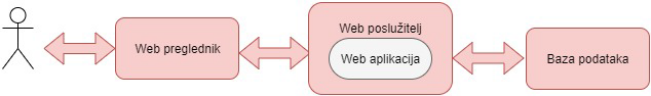
\includegraphics[width=.9\linewidth]{slike/arhitektura_sustava.png}
			\centering
			\caption{Arhitektura sustava}
			\label{fig:arh1}
		\end{figure}

		\indent \underline{\textit{Web preglednik}} (internetski preglednik) program je koji omogućuje korisnicima pristup web stranicama i multimedijalnim sadržajima vezanih uz njih. Svaki internetski preglednik je prevoditelj što znači da je stranica pisana u kodu koji se potom interpretira kao nešto svakome razumljivo. Putem web preglednika korisnik šalje zahtjeve web poslužitelju. \\
		\indent \underline{\textit{Web poslužitelj}} je računalni program koji služi kao medij između korisnika i drugih programa ili uređaja. Poslužitelj je osnova rada web aplikacije budući da on pokreće web aplikaciju te joj preusmjerava zahtjeve klijenata. Njegova primarna funkcija je pohranjivanje, obrada i isporuka web stranica klijentima. Komunikacija izmedu klijenta i poslužitelja odvija se pomoću protokola HTTP (engl. \textit{Hyper Text Transfer Protocol}).\\
		\indent \underline{\textit{Web aplikacija}} je računalni program kojemu klijent pristupa iz web preglednika za obradu željenih zahtjeva. Ovisno o tipu zahtjeva, aplikacija pristupa bazi podataka zatim preko poslužitelja vraća korisniku odgovor vidljiv u web pregledniku kao HTML dokument.\\
		
		Programski jezik koji smo koristili za izradu web aplikacije "Maketa Shop" je Python s Flask radnim okvirom.\\
		
		MVC (Model-View-Controller) je obrazac koji se obično koristi za razvoj korisničkih sučelja zato jer dijeli programsku	logiku na tri medusobno povezana elementa što pojednostavnjuje razvoj web	aplikacija. Flask nije strukuriran kao čisti MVC okvir, ali po funkcionalnosti je vrlo sličan. Stoga možemo definirati sva tri elementa: 
		\begin{itemize}
			\item Model --- Središnja komponenta sustava.To je dinamička struktura podataka aplikacije neovisna o korisničkom sučelju. Izravno upravlja podacima, logikom i pravilima aplikacije i prima podatke od Controllera.
			\item View --- Svako predstavljanje informacija poput grafova, dijagrama ili tablica. Moguće je višestruko prikazivanje istih podataka, poput trake grafikona za upravljanje i tabličnog prikaza.
			\item Controller --- Prihvaća unos i pretvara ga u naredbe za Model ili View. Upravlja	korisničkim zahtjevima te izvodi daljnju interakciju.
		\end{itemize}
				
		\section{Baza podataka}
			
			\noindent Sutav koristi relacijsku bazu podataka. Baza se sastoji od relacija, tablica koje svojim atributima modeliraju pojave iz stvarnog svijeta. Uloga baze je strukurirana pohrana  podataka radi njihova lakšeg dohvaćanja i izmjenjivanja. Baza ovog sustava se sadrži od sljedećih entiteta:
			\begin{itemize}
				\item User (korisnik)
				\item Banned (blokirani korisnici)
				\item Profile (osobni podaci korisnika)
				\item BillingInfo (podaci o plaćanju)
				\item Story (priča)
				\item StoryContent (dio sadržaja priče) 
				\item Model (maketa)
				\item ModelPhoto (fotografija koja se prilaže maketi)
				\item ModelPrice (cijena modela ovisno o materijalu)
				\item ModelNotification (obavijest)
				\item Comment (komentar)
				\item Order (narudžba)
				\item OrderModel (makete po narudžbi)
				\item Cart (košarica)
				\item CartModel (model u košarici)
			\end{itemize}
		
			\subsection{Opis tablica}
			

				\noindent\textbf{User}  Podaci potrebni za prijavu u sustav. Sadrži atribute: identifikacijski broj, korisničko ime, e-mail adresu i lozinku. U vezi je \textit{One-to-One} s entitetom BillingInfo preko atributa id, u vezi \textit{One-to-One} s entitetom Profile preko atributa id, u vezi \textit{One-to-Many} s entitetom Story preko atributa id, u vezi \textit{One-to-Many} s entitetom Order preko atributa id, u vezi \textit{One-to-Many} s entitetom Model preko atributa id, u vezi \textit{One-to-Many} s entitetom Cart preko atributa id, u vezi \textit{One-to-Many} s entitetom Model preko atributa id, u vezi \textit{One-to-Many} s entitetom Comment preko atributa id, u vezi \textit{One-to-Many} s entitetom ModelNotification preko atributa id.

				\begin{longtabu} to \textwidth {|X[6, l]|X[6, l]|X[20, l]|}
					
					\hline \multicolumn{3}{|c|}{\textbf{User}}	 \\[3pt] \hline
					\endfirsthead
					
					\hline \multicolumn{3}{|c|}{\textbf{User}}	 \\[3pt] \hline
					\endhead
					
					\hline 
					\endlastfoot
					
					\cellcolor{LightGreen} id& INT	&  identifikacijski broj korisnika; samoinkrementirajući broj jedinstven za svakog korisnika	\\ \hline
					username& VARCHAR &  ime koje se prikazuje drugim korisnicima; jedinstveno 	\\ \hline 
					email & VARCHAR & E-mail adresa kojom se prijavljuje u sustav; jedinstvena  \\ \hline 
					password & CHAR & lozinka kojem se prijavljuje u sustav, kriptirana algoritmom Bcrypt na 60 bajtova \\ \hline

				\end{longtabu}
			
				\noindent\textbf{Profile} Podaci koje korisnik može prikazati na svom profilu. Sadrži atribute: ime, prezime, datum rođenja, kratak životopis, te postavke privatnosti za svaku od stavki. U vezi \textit{One-to-One} s entitetom User.
			
				\begin{longtabu} to \textwidth {|X[6, l]|X[6, l]|X[20, l]|}
				
					\hline \multicolumn{3}{|c|}{\textbf{Profile}}	 \\[3pt] \hline
					\endfirsthead
					
					\hline \multicolumn{3}{|c|}{\textbf{Profile}}	 \\[3pt] \hline
					\endhead
					
					\hline 
					\endlastfoot
					
					\cellcolor{LightGreen} user\_id& INT	&  identifikacijski broj korisnika kojemu profil pripada \\ \hline
					first\_name & VARCHAR &  korisnikovo ime; opcionalno	\\ \hline 
					private\_name & BOOLEAN & TRUE ako je javno, FALSE ako nije \\ \hline
					last\_name & VARCHAR & korisnikovo prezime; opcionalno  \\ \hline 
					private\_lname & BOOLEAN & TRUE ako je javno, FALSE ako nije \\ \hline
					DOB & DATETIME & korisnikov datum rođenja; opcionalno \\ \hline
					private\_DOB & BOOLEAN & TRUE ako je javno, FALSE ako nije \\ \hline
					bio & TEXT	& kratak životopis; opcionalno\\ \hline 
					private\_bio & BOOLEAN & TRUE ako je javno, FALSE ako nije \\ \hline
				
				\end{longtabu}
			
				\noindent\textbf{BillingInfo} Sadrži korisnikove podatke o plaćanju. Sadrži atribute: puno ime, adresa za naplatu, broj kreditne kartice, datum isteka kartice, CVC kartice, državu, puno ime kartice, zip kod i email adresu. U vezi \textit{One-to-One} s entitetom User.
			
				\begin{longtabu} to \textwidth {|X[6, l]|X[6, l]|X[20, l]|}
	
					\hline \multicolumn{3}{|c|}{\textbf{BillingInfo}}	 \\[3pt] \hline
					\endfirsthead
					
					\hline \multicolumn{3}{|c|}{\textbf{BillingInfo}}	 \\[3pt] \hline
					\endhead
					
					\hline 
					\endlastfoot
					
					\cellcolor{LightGreen} user\_id& INT	&  identifikacijski broj korisnika kojemu podaci pripadaju \\ \hline
					full\_name & VARCHAR &  korisnikovo ime i prezime	\\ \hline 
					email & VARCHAR & email adresa korisnika  \\ \hline 
					address & VARCHAR & adresa\\ \hline
					country & VARCHAR & država\\ \hline
					city & VARCHAR & grad\\ \hline
					zip\_code & VARCHAR & poštanski broj\\ \hline
					card\_full\_name & VARCHAR & puno ime kreditne kartice \\ \hline
					card\_number & VARCHAR & broj kreditne kartice \\ \hline
					card\_expiry & DATETIME & datum isteka kartice \\ \hline
					card\_CVC & INT & CVC kartice \\ \hline
					
				\end{longtabu}
			
				\noindent\textbf{Story} Osnovne informacije o priči koju korisnik postavlja na aplikaciju. Sadrži atribute: identifikacijski broj, naslov priče, vrijeme nastanka, stanje (prihvaćena / neprihvaćena) i identifikacijski broj autora. U vezi je \textit{One-to-Many} s entitetom StoryContent te u vezi \textit{Many-to-One} s entitetom User.
			
				\begin{longtabu} to \textwidth {|X[6, l]|X[6, l]|X[20, l]|}
				
					\hline \multicolumn{3}{|c|}{\textbf{Story}}	 \\[3pt] \hline
					\endfirsthead
					
					\hline \multicolumn{3}{|c|}{\textbf{Story}}	 \\[3pt] \hline
					\endhead
					
					\hline 
					\endlastfoot
					
					\cellcolor{LightGreen} id& INT	&  identifikacijski broj priče; samoinkrementirajući broj jedinstven za svaku priču	\\ \hline
					title& TEXT &  naslov priče \\ \hline 
					time\_created & DATETIME & vrijeme nastanka priče \\ \hline 
					validated & BOOLEAN & TRUE ako je priča prhvaćena, FALSE ako nije \\ \hline
					\cellcolor{LightBlue}author\_id & INT & identifikacijski broj autora \\ \hline 
				
				\end{longtabu}
			
				\noindent\textbf{StoryContent} Tekst, slika ili video koji se prilaže priči. Sadrži atribute: identifikacijski broj priče, redni broj dijela sadržaja, tekst priče, ime slike i ime videa.
				U vezi je \textit{Many-to-One} s entitetom Story.
				
				\begin{longtabu} to \textwidth {|X[6, l]|X[6, l]|X[20, l]|}
					
					\hline \multicolumn{3}{|c|}{\textbf{StoryContent}}	 \\[3pt] \hline
					\endfirsthead
					
					\hline \multicolumn{3}{|c|}{\textbf{StoryContent}}	 \\[3pt] \hline
					\endhead
					
					\hline 
					\endlastfoot
					
					\cellcolor{LightGreen} story\_id & INT &  identifikacijski broj priče kojemu se sadržaj prilaže \\ \hline
					\cellcolor{LightGreen}ordinal\_number & INT &  redni broj dijela sadržaja u priči	\\ \hline 
					story\_text & TEXT & tekst koji se prilaže priči; opcionalno \\ \hline 
					image\_name & VARCHAR & ime slike koja se prilaže priči; opcionalno \\ \hline
					video\_name & VARCHAR &  ime videa koji se prilaže priči, opcionalno \\ \hline 
					
				\end{longtabu}
			
				\noindent\textbf{Model} Podaci o maketi koju predlaže korisnik. Sadrži atribute: identifikacijski broj, ime, opis, identifikacijski broj korisnika koji ju predlaže, dimenzije, boje i odobrenost. U vezi je \textit{Many-to-One} s entitetom User, u vezi \textit{One-to-Many} s entitetom ModelPrice, u vezi \textit{One-to-Many} s entitetom ModelPhoto, u vezi \textit{Many-to-Many} s entitetom Order-Model te u vezi \textit{One-to-Many} s entitetom CartModel.
				
				\begin{longtabu} to \textwidth {|X[6, l]|X[6, l]|X[20, l]|}
					
					\hline \multicolumn{3}{|c|}{\textbf{Model}}	 \\[3pt] \hline
					\endfirsthead
					
					\hline \multicolumn{3}{|c|}{\textbf{Model}}	 \\[3pt] \hline
					\endhead
					
					\hline 
					\endlastfoot
					
					\cellcolor{LightGreen} id & INT &  identifikacijski broj makete; samoinkrementirajući broj jedinstven za svaku maketu \\ \hline
					name & VARCHAR &  ime makete; jedinstveno	\\ \hline 
					description & TEXT & opis makete \\ \hline 
					dimension & VARCHAR &  dimenzije; odvojene znakom ","	\\ \hline 
					colors & VARCHAR &  dostupne boje; odvojene znakom ","	\\ \hline 
					approved & BOOLEAN & TRUE ako je model prhvaćen, FALSE ako nije \\ \hline
					\cellcolor{LightBlue} creator\_id & INT & identifikacijski broj korisnika koji predlaže maketu \\ \hline
					
				\end{longtabu}
			
				\noindent\textbf{ModelPhoto} Fotografija koja se prilaže maketi. Sadrži atribute: ime slike i identifikacijski broj makete. U vezi \textit{Many-to-One} s entitetom Model.
				
				\begin{longtabu} to \textwidth {|X[6, l]|X[6, l]|X[20, l]|}
					
					\hline \multicolumn{3}{|c|}{\textbf{ModelPhoto}}	 \\[3pt] \hline
					\endfirsthead
					
					\hline \multicolumn{3}{|c|}{\textbf{ModelPhoto}}	 \\[3pt] \hline
					\endhead
					
					\hline 
					\endlastfoot
					
					\cellcolor{LightGreen} image\_name & VARCHAR & ime fotografije \\ \hline
					\cellcolor{LightBlue} model\_id & INT & identifikacijski broj makete kojemu se fotografija prilaže \\ \hline
					
				\end{longtabu}
			
				\noindent\textbf{ModelPrice} Cijena makete ovisno o materijalu od kojeg je izrađena. Sadrži atribute: identifijacijski broj modela, materijal od kojeg je izrađena, cijenu makete te samoinkrementirajući id makete.
				U vezi \textit{Many-to-One} s entitetom Model.
				
				\begin{longtabu} to \textwidth {|X[6, l]|X[6, l]|X[20, l]|}
					
					\hline \multicolumn{3}{|c|}{\textbf{ModelPrice}}	 \\[3pt] \hline
					\endfirsthead
					
					\hline \multicolumn{3}{|c|}{\textbf{ModelPrice}}	 \\[3pt] \hline
					\endhead
					
					\hline 
					\endlastfoot
					
					\cellcolor{LightGreen} model\_id & INT & identifikacijski broj makete \\ \hline
					\cellcolor{LightGreen} material & VARCHAR & ime materijala \\ \hline
					price & NUMERIC & cijena makete za zadani materijal \\ \hline
					id & INT &  identifikacijski broj; samoinkrementirajući broj jedinstven za svaku instancu ModelPrice \\ \hline
					
				\end{longtabu}
			
				\noindent\textbf{Order} Podaci o narudžbi koju korisnik šalje trgovini. Sadrži atribute: identifikacijski broj narudžbe, vrijeme nastanka, identifikacijski broj korisnika koji šalje narudžbu te ime, adresu i email kupca. U vezi je \textit{Many-to-One} s entitetom User i u vezi \textit{One-to-Many} s entitetom OrderModel.
				
				\begin{longtabu} to \textwidth {|X[6, l]|X[6, l]|X[20, l]|}
					
					\hline \multicolumn{3}{|c|}{\textbf{Order}}	 \\[3pt] \hline
					\endfirsthead
					
					\hline \multicolumn{3}{|c|}{\textbf{Order}}	 \\[3pt] \hline
					\endhead
					
					\hline 
					\endlastfoot
					
					\cellcolor{LightGreen} id & INT &  identifikacijski broj narudžbe; samoinkrementirajući broj jedinstven za svaku narudžbu \\ \hline
					time\_created & DATETIME &  vrijeme nastanka	\\ \hline 
					buyer\_name & VARCHAR & ime kupca \\ \hline
					buyer\_email & VARCHAR & email adresa kupca \\ \hline
					buyer\_address & VARCHAR & adresa kupca \\ \hline
					\cellcolor{LightBlue} user\_id & INT & identifikacijski broj korisnika koji šalje narudžbu \\ \hline
					
				\end{longtabu}
			
				\noindent\textbf{OrderModel} Lista maketa u narudžbi. Sadrži atribute: identifikacijski broj narudžbe, identifikacijski broj makete, materijal od kojeg je maketa izrađena količinu i cijena makete u trenutku narudžbe.
				
				\begin{longtabu} to \textwidth {|X[6, l]|X[6, l]|X[20, l]|}
					
					\hline \multicolumn{3}{|c|}{\textbf{OrderModel}}	 \\[3pt] \hline
					\endfirsthead
					
					\hline \multicolumn{3}{|c|}{\textbf{OrderModel}}	 \\[3pt] \hline
					\endhead
					
					\hline 
					\endlastfoot
					
					\cellcolor{LightBlue} order\_id & INT &  identifikacijski broj narudžbe \\ \hline
					\cellcolor{LightBlue} model\_id & INT & identifikacijski broj makete \\ \hline
					material & VARCHAR & ime materijala od kojeg je maketa izrađena \\ \hline
					price & NUMERIC & cijena makete za zadani materijal u trenutku narudžbe \\ \hline
					quantity & INT & količina makete \\ \hline
					
				\end{longtabu}

				\noindent\textbf{Comment} Komentari ispod pojedine priče, u vezi \textit{Many-to-One} s entitetom User te u vezi \textit{Many-to-One} s entitetom Story.
				
				\begin{longtabu} to \textwidth {|X[6, l]|X[6, l]|X[20, l]|}
					
					\hline \multicolumn{3}{|c|}{\textbf{Comment}}	 \\[3pt] \hline
					\endfirsthead
					
					\hline \multicolumn{3}{|c|}{\textbf{Comment}}	 \\[3pt] \hline
					\endhead
					
					\hline 
					\endlastfoot
					
					\cellcolor{LightBlue} id & INT &  identifikacijski broj komentara \\ \hline
					\cellcolor{LightBlue} id & INT &  identifikacijski broj priče \\ \hline
					\cellcolor{LightBlue} author\_id & INT & identifikacijski broj autora komentara \\ \hline
					text & TEXT & tekst komentara \\ \hline
					timestamp & DATETIME & vrijeme nastanka komentara \\ \hline 
					
				\end{longtabu}

				\noindent\textbf{ModelNotification} Obavijest o prihvaćanju naručene makete, u vezi \textit{Many-to-One} s entitetom Model te u vezi \textit{Many-to-One} s entitetom User.
				
				\begin{longtabu} to \textwidth {|X[6, l]|X[6, l]|X[20, l]|}
					
					\hline \multicolumn{3}{|c|}{\textbf{ModelNotification}}	 \\[3pt] \hline
					\endfirsthead
					
					\hline \multicolumn{3}{|c|}{\textbf{ModelNotification}}	 \\[3pt] \hline
					\endhead
					
					\hline 
					\endlastfoot
					
					\cellcolor{LightBlue} id & INT &  identifikacijski broj obavijesti \\ \hline
					\cellcolor{LightBlue} receiver\_id & INT &  identifikacijski broj primatelja obavijesti \\ \hline
					\cellcolor{LightBlue} model\_id & INT & identifikacijski broj naručenog modela \\ \hline
					seen & BOOLEAN & pregledanost obavijesti \\ \hline
					time\_create & DATETIME & vrijeme nastanka obavijesti \\ \hline 
					
				\end{longtabu}

				\noindent\textbf{Cart} Entitet košarice pridružen entitetu User vezom \textit{One-to-One}.
				
				\begin{longtabu} to \textwidth {|X[6, l]|X[6, l]|X[20, l]|}
					
					\hline \multicolumn{3}{|c|}{\textbf{Cart}}	 \\[3pt] \hline
					\endfirsthead
					
					\hline \multicolumn{3}{|c|}{\textbf{Cart}}	 \\[3pt] \hline
					\endhead
					
					\hline 
					\endlastfoot
					
					\cellcolor{LightBlue} buyer\_id & INT &  identifikacijski broj kupca \\ \hline
					
				\end{longtabu}

				\noindent\textbf{CartModel} Lista maketa u košarici. Sadrži atribute: identifikacijski broj košarice, identifikacijski broj makete, materijal od kojeg je maketa izrađena te količinu i cijenu makete u košarici, u vezi \textit{Many-to-One} s entitetom Cart.
				
				\begin{longtabu} to \textwidth {|X[6, l]|X[6, l]|X[20, l]|}
					
					\hline \multicolumn{3}{|c|}{\textbf{CartModel}}	 \\[3pt] \hline
					\endfirsthead
					
					\hline \multicolumn{3}{|c|}{\textbf{CartModel}}	 \\[3pt] \hline
					\endhead
					
					\hline 
					\endlastfoot
					
					\cellcolor{LightBlue} cart\_id & INT &  identifikacijski broj košarice \\ \hline
					\cellcolor{LightBlue} model\_id & INT & identifikacijski broj makete \\ \hline
					material & VARCHAR & ime materijala od kojeg je maketa izrađena \\ \hline
					price & NUMERIC & cijena makete za zadani materijal u košarici \\ \hline
					quantity & INT & količina maketa \\ \hline
					
				\end{longtabu}
			
			\subsection{Dijagram baze podataka}
				\begin{figure}[H]
					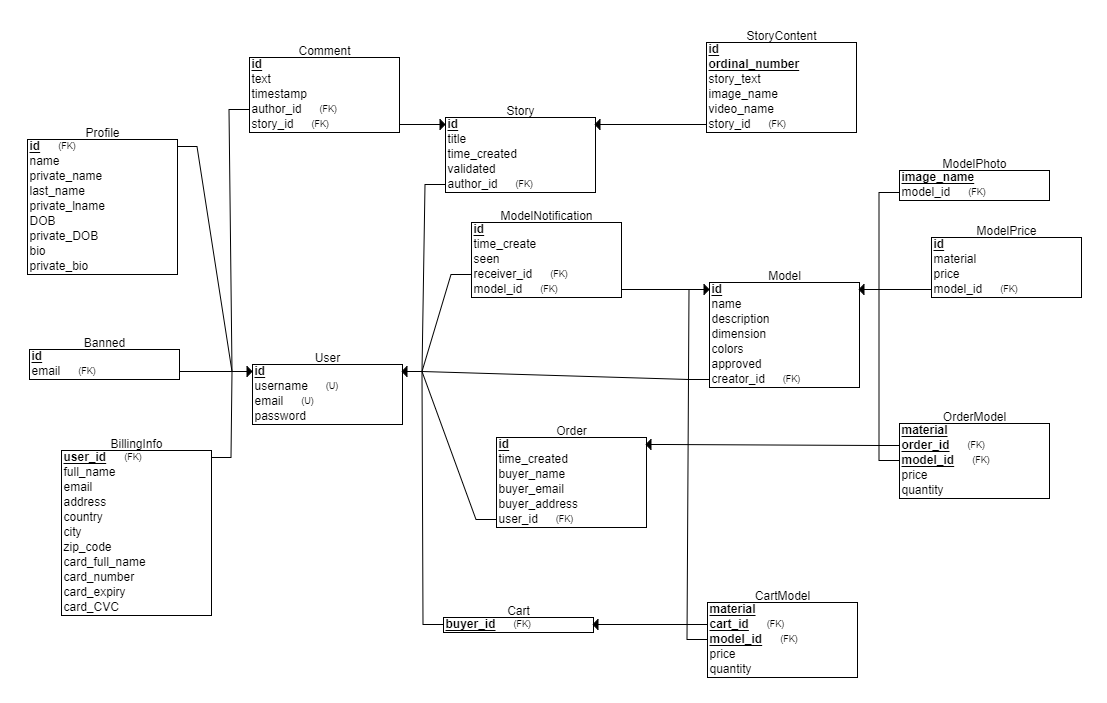
\includegraphics[width=1\linewidth]{dijagrami/ER_baza_podataka.PNG}
					\caption{E-R dijagram baze podataka}
					\label{fig:erdija}
				\end{figure}
			\eject
			
			
		\section{Dijagram razreda}
				
			\begin{figure}[H]
				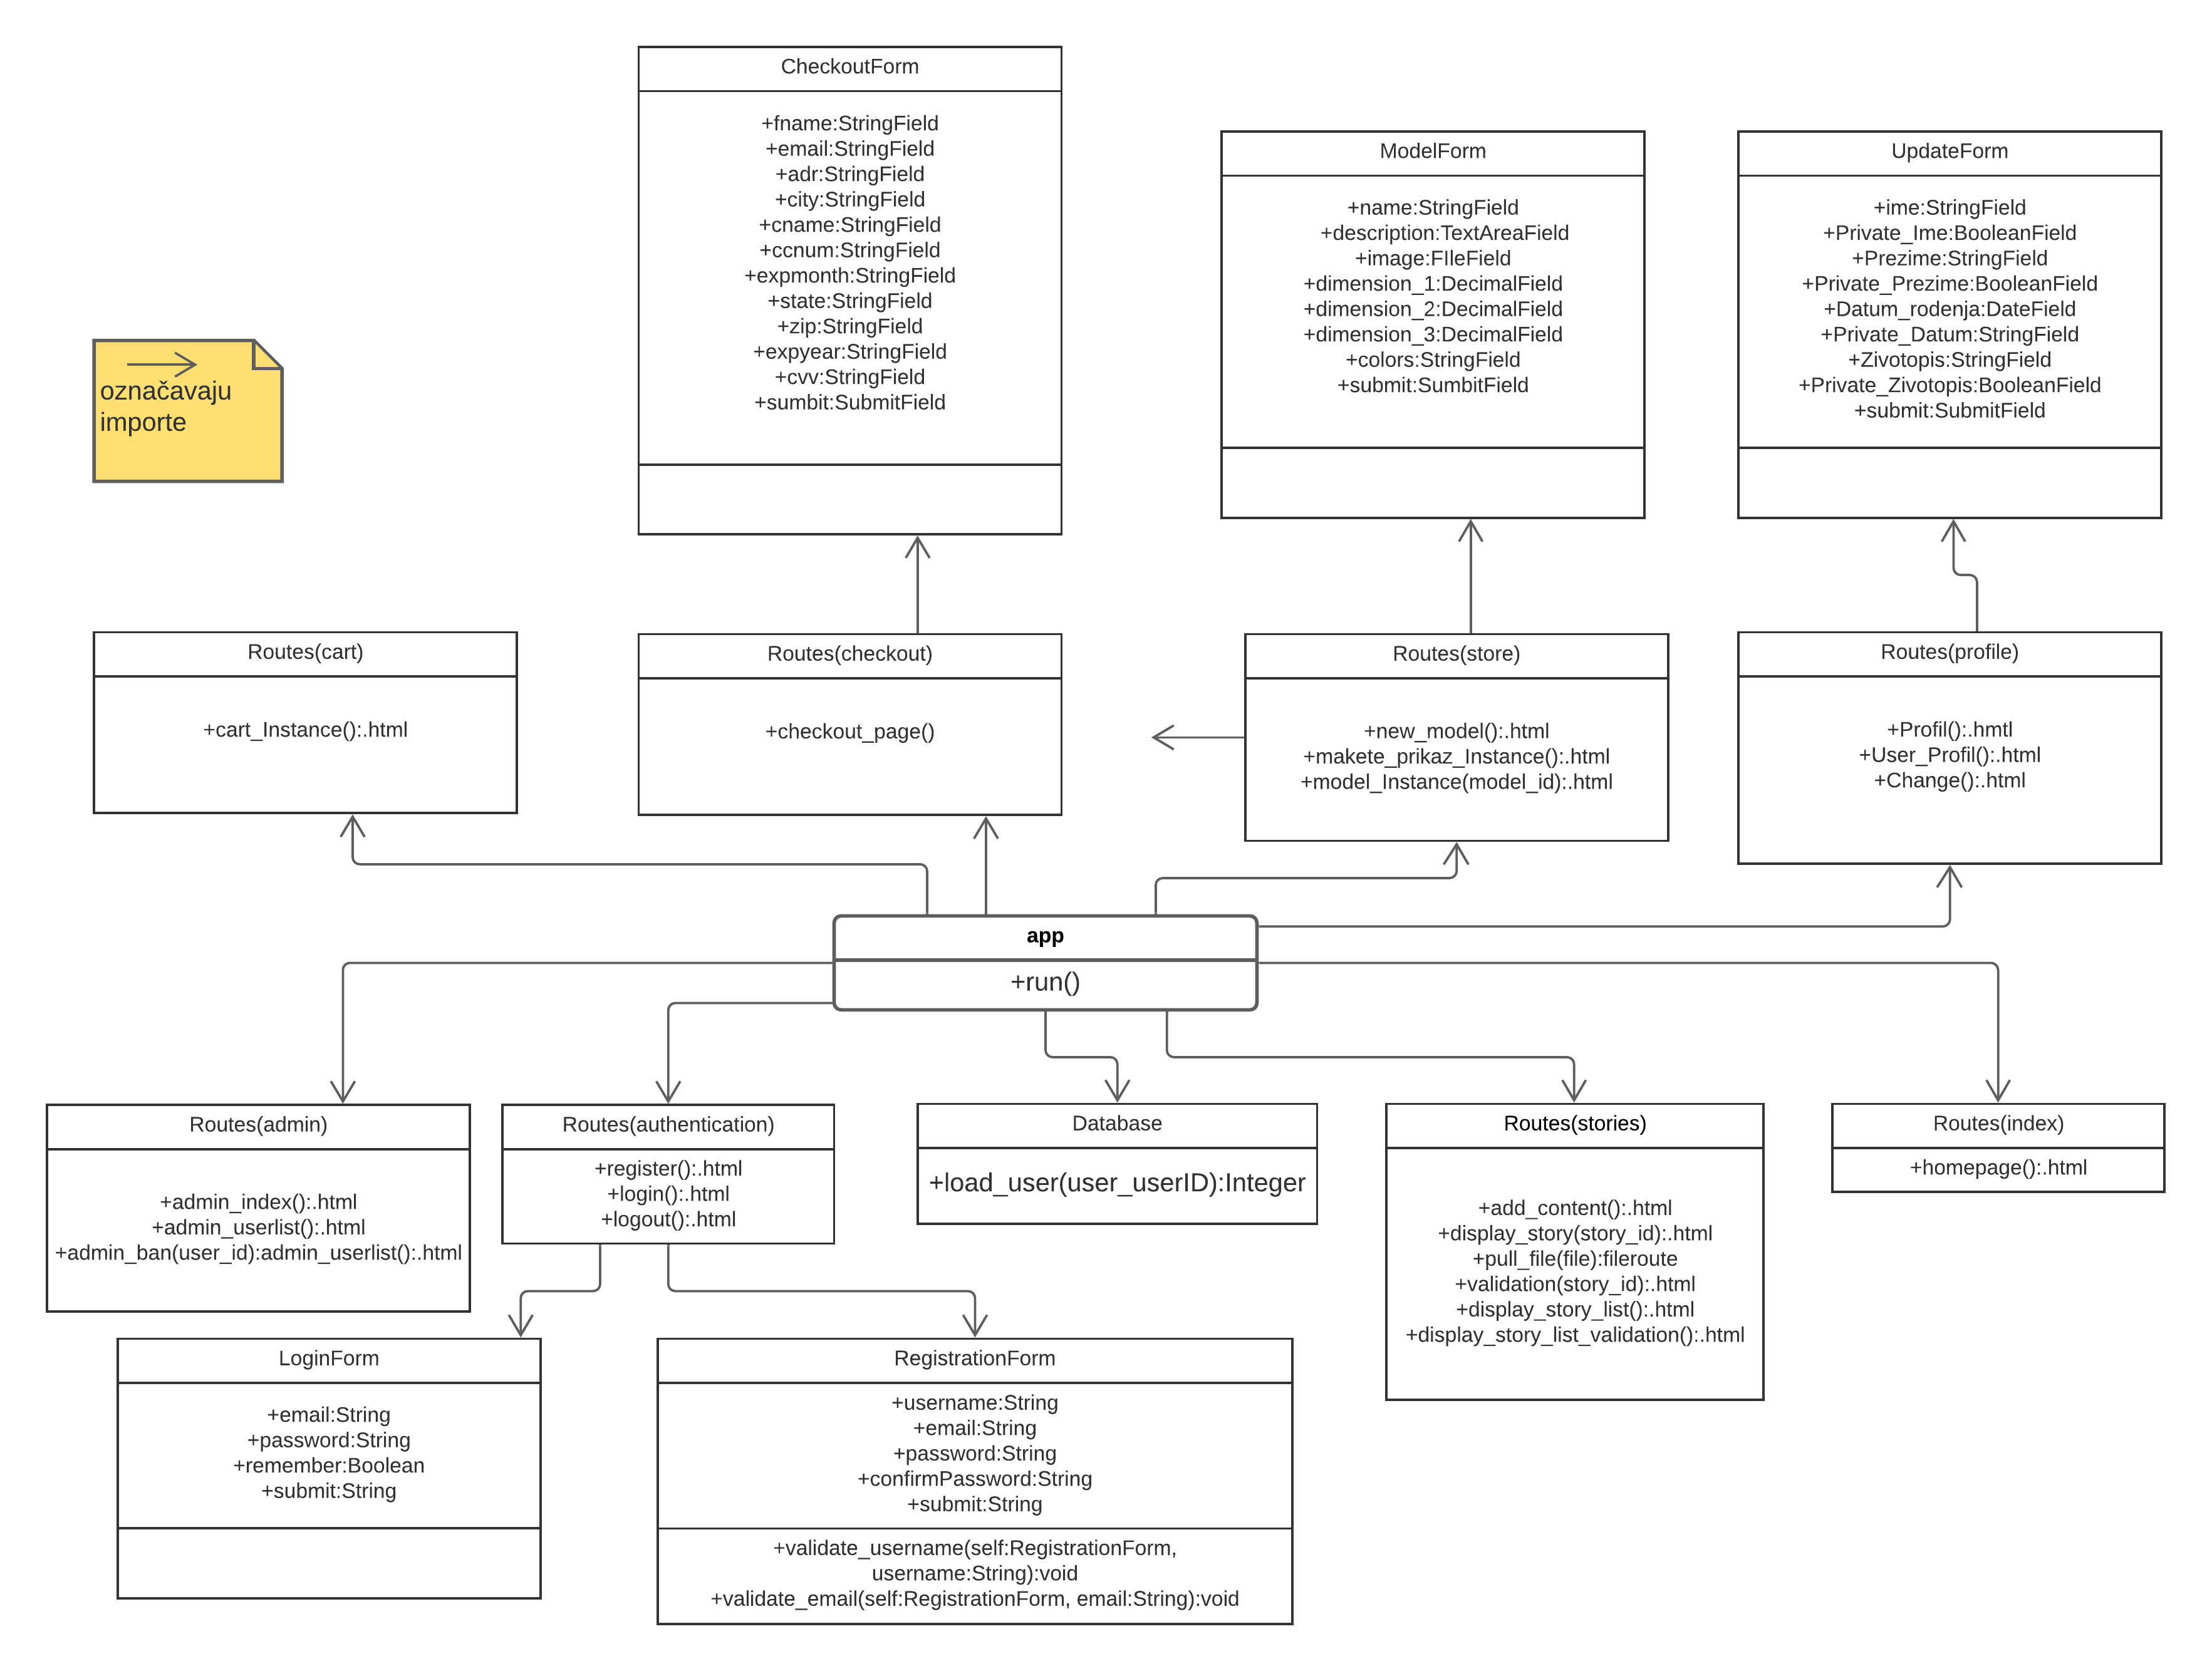
\includegraphics[width=.9\linewidth]{slike/Dijagram_razreda.PNG} %veličina u odnosu na širinu linije
				\caption{Dijagram razreda}
				\label{fig:diraz1} %label mora biti drugaciji za svaku sliku
			\end{figure}
		
			Razredi vezani uz bazu podataka su smješteni na zasebnoj slici zbog lakše preglednosti.
		
			\begin{figure}[H]
				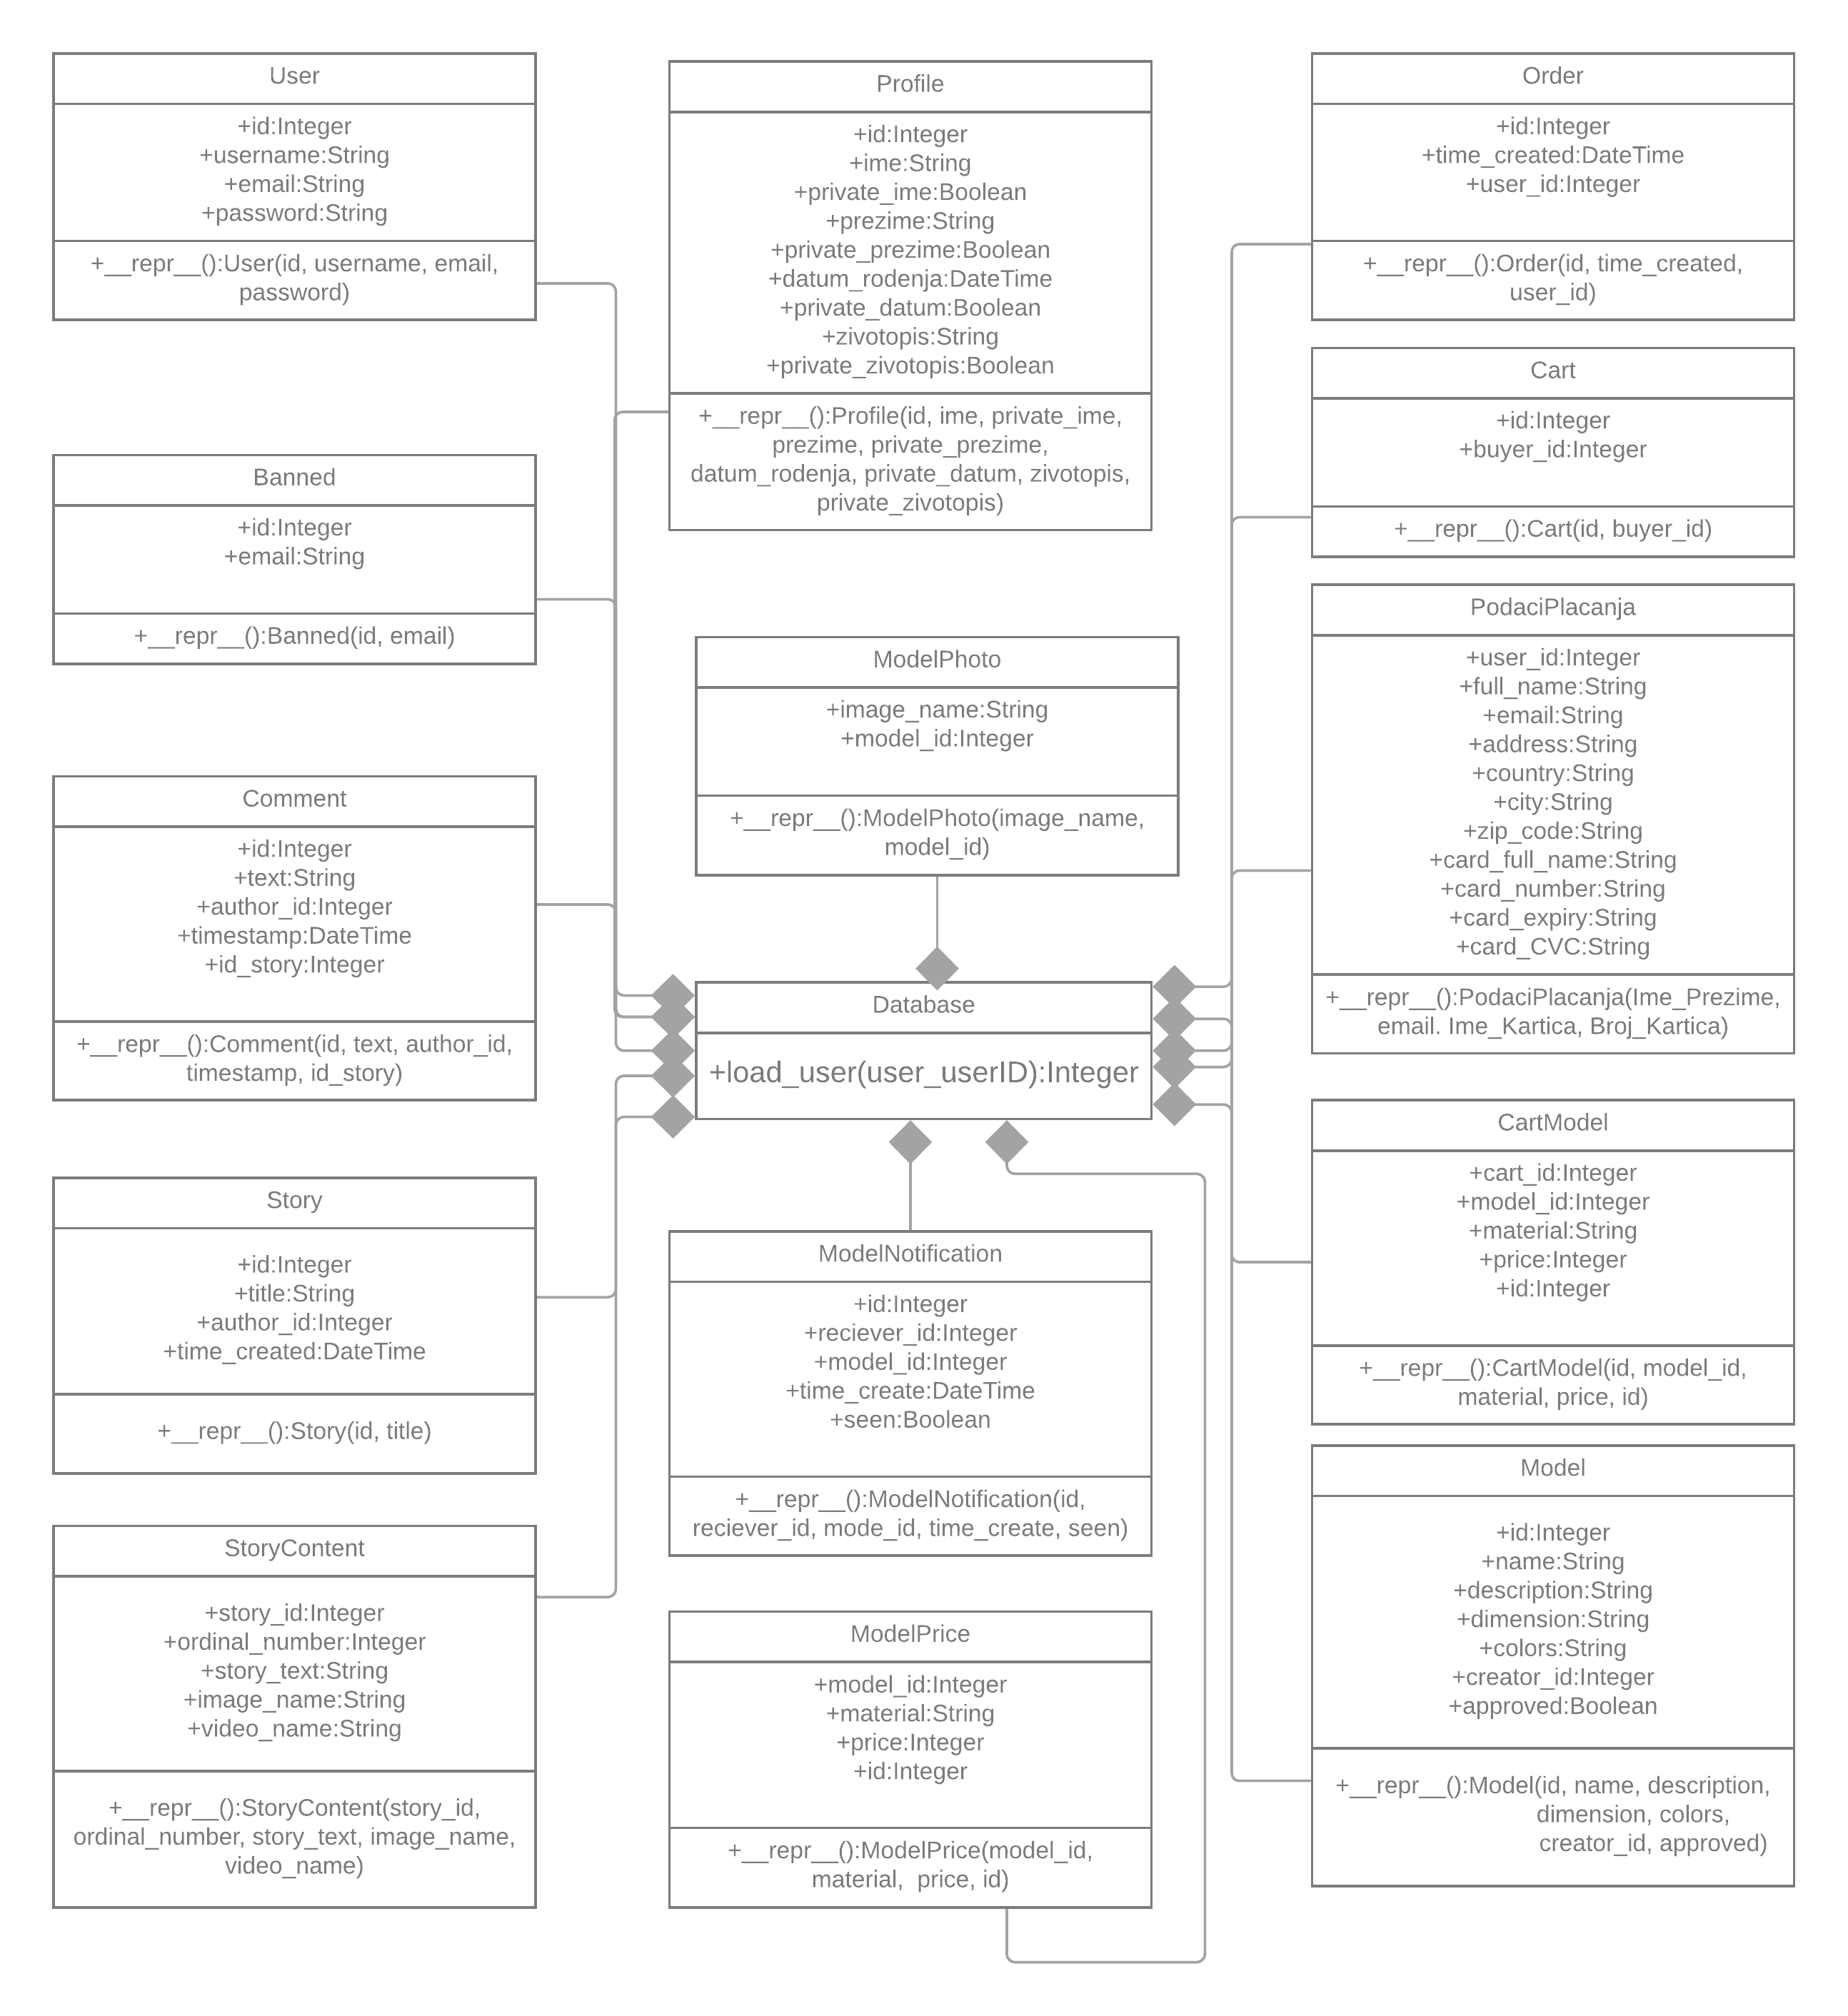
\includegraphics[width=.9\linewidth]{slike/Dijagram_razreda_baza.PNG} %veličina u odnosu na širinu linije
				\caption{Dijagram razreda - Baza podataka}
				\label{fig:diraz2} %label mora biti drugaciji za svaku sliku
			\end{figure}
		
		\section{Dijagram stanja}
			
			
			Dijagram stanja opisuje dinamičko ponašanje dijela sustava u vremenu. Njim se prikazuj stanje objekta te prijelazi iz jednog stanja u drugo temeljeni na događajima. Na slici ispod prikazan je dijagram stanja za prijavljenog korisnika u sustav. Korisniku se pri otvaranju stranice prikazuje početna stranica te dalje pomoću izbornika u zaglavlju pristupa funkcijama koje mu se nude. Prijavljeni korisnik može pregledavati, komentirati i predlagati priče. Također, može pregledavati standardne makete u sustavu i kupovati ih ili naručiti maketu po svojim zahtjevima. Klikom na "Korisnički račun" u izborniku korisniku se daje pregled njegovog računa sa mogučnošću izmjene podataka i vidljivosti svakog podatka. Na kraju, korisnik također može pristupiti svojoj košarici i preko nje dovršiti kupnju.
			
			\begin{figure}[H]
				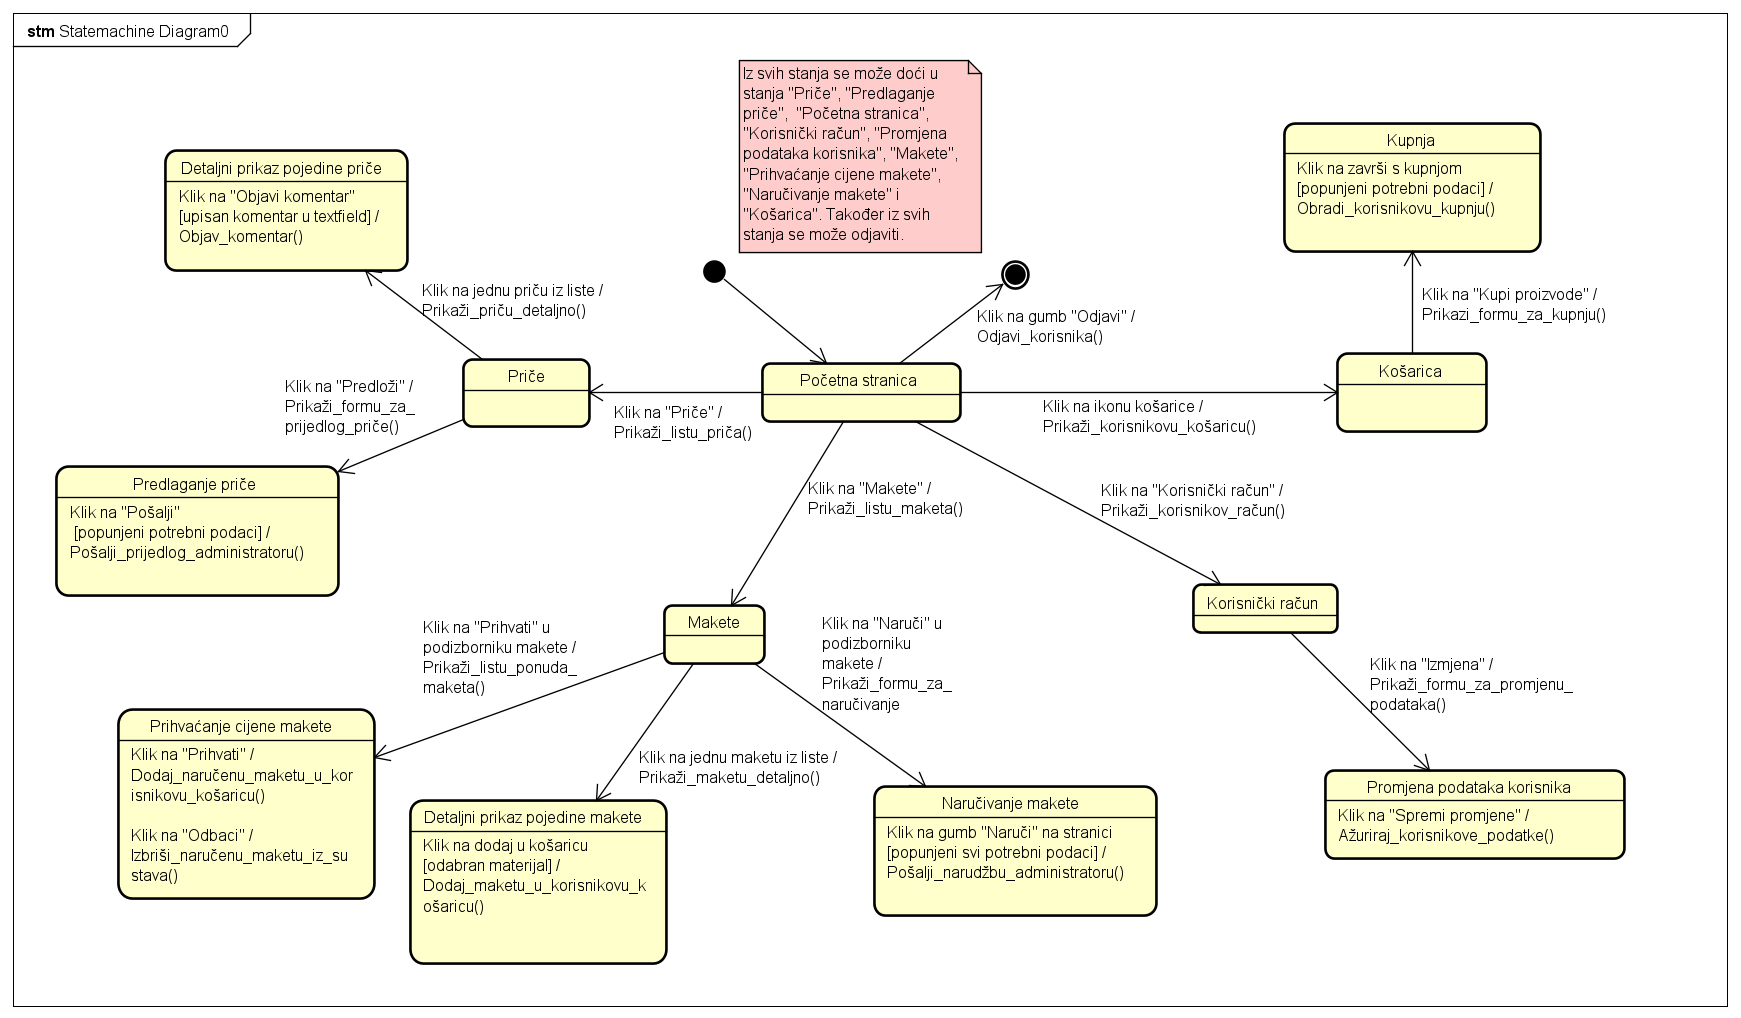
\includegraphics[width=1\linewidth]{slike/Dijagram_stanja.PNG} %veličina u odnosu na širinu linije
				\caption{Dijagram stanja}
				\label{fig:dijstan} %label mora biti drugaciji za svaku sliku
			\end{figure}
			
			
			\eject 
		
		\section{Dijagram aktivnosti}
			
			\begin{figure}[H]
				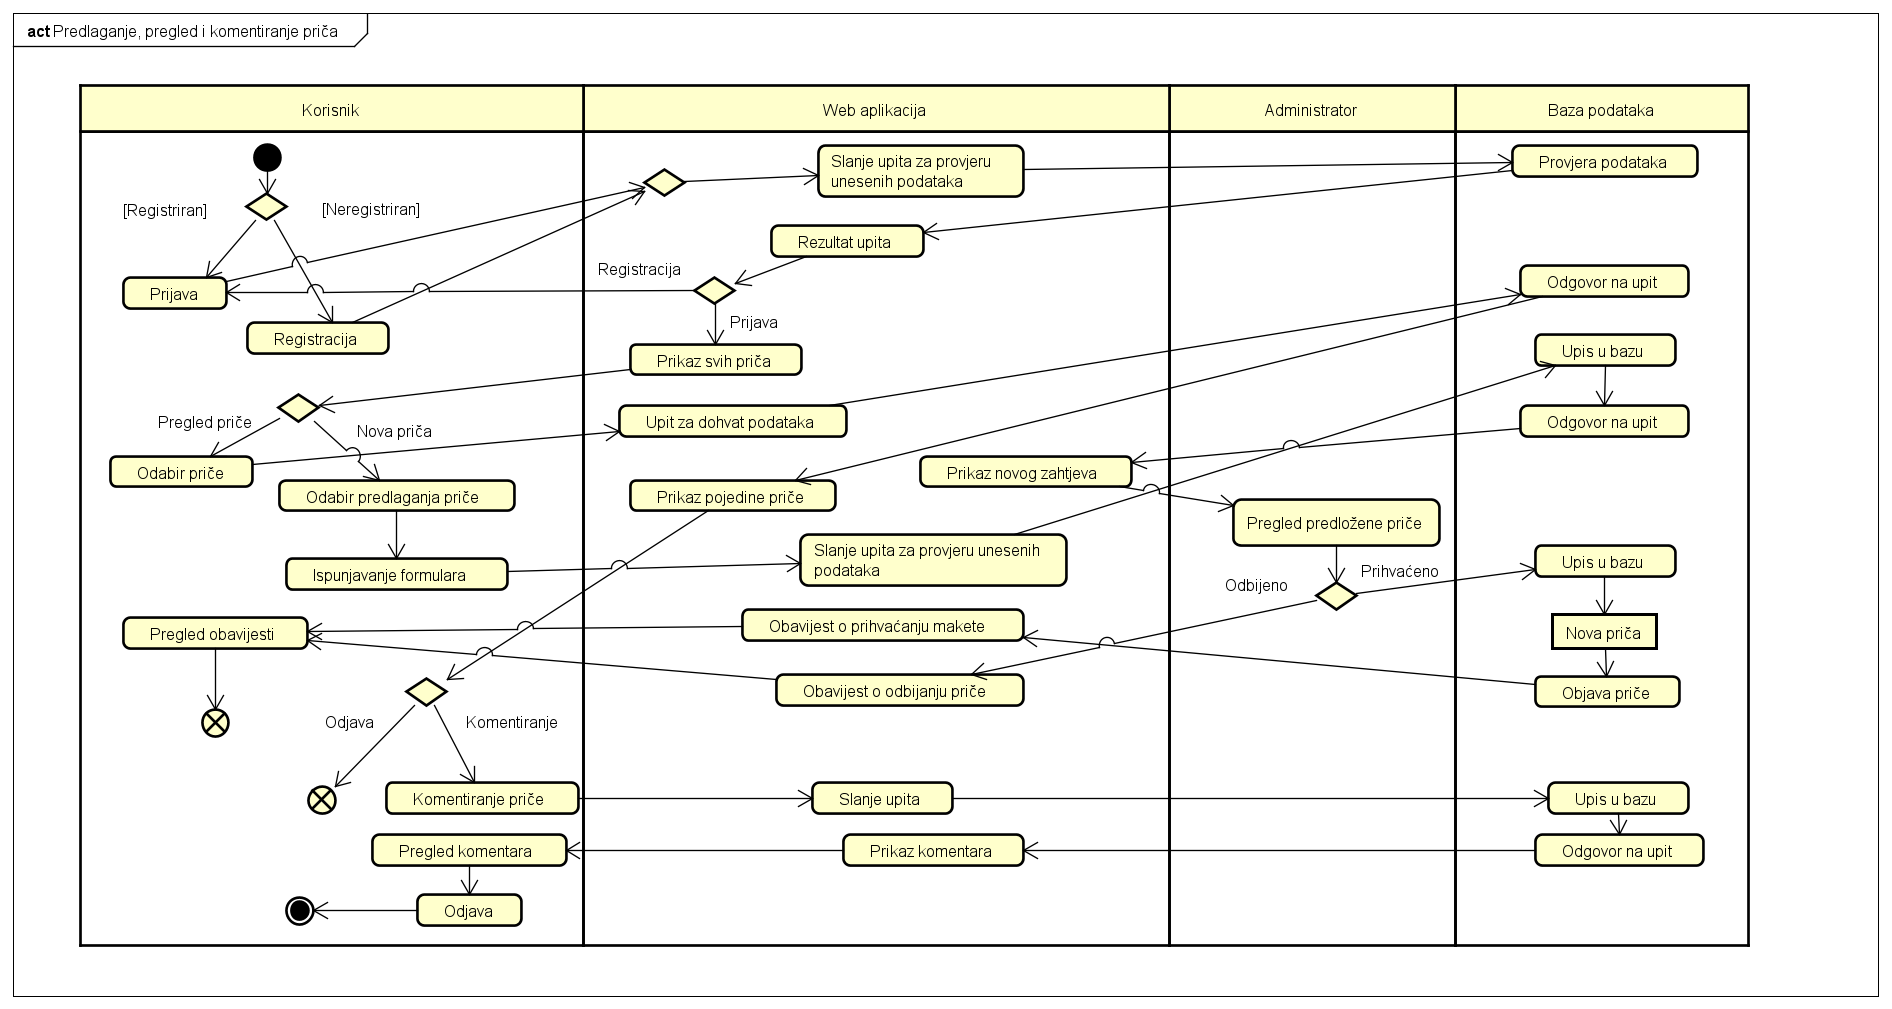
\includegraphics[width=1\linewidth]{slike/Dijagram_aktivnosti_1.PNG} %veličina u odnosu na širinu linije
				\caption{Dijagram aktivnosti za predlaganje, pregled i komentiranje priča}
				\label{fig:diakt1} %label mora biti drugaciji za svaku sliku
			\end{figure}

			\begin{figure}[H]
				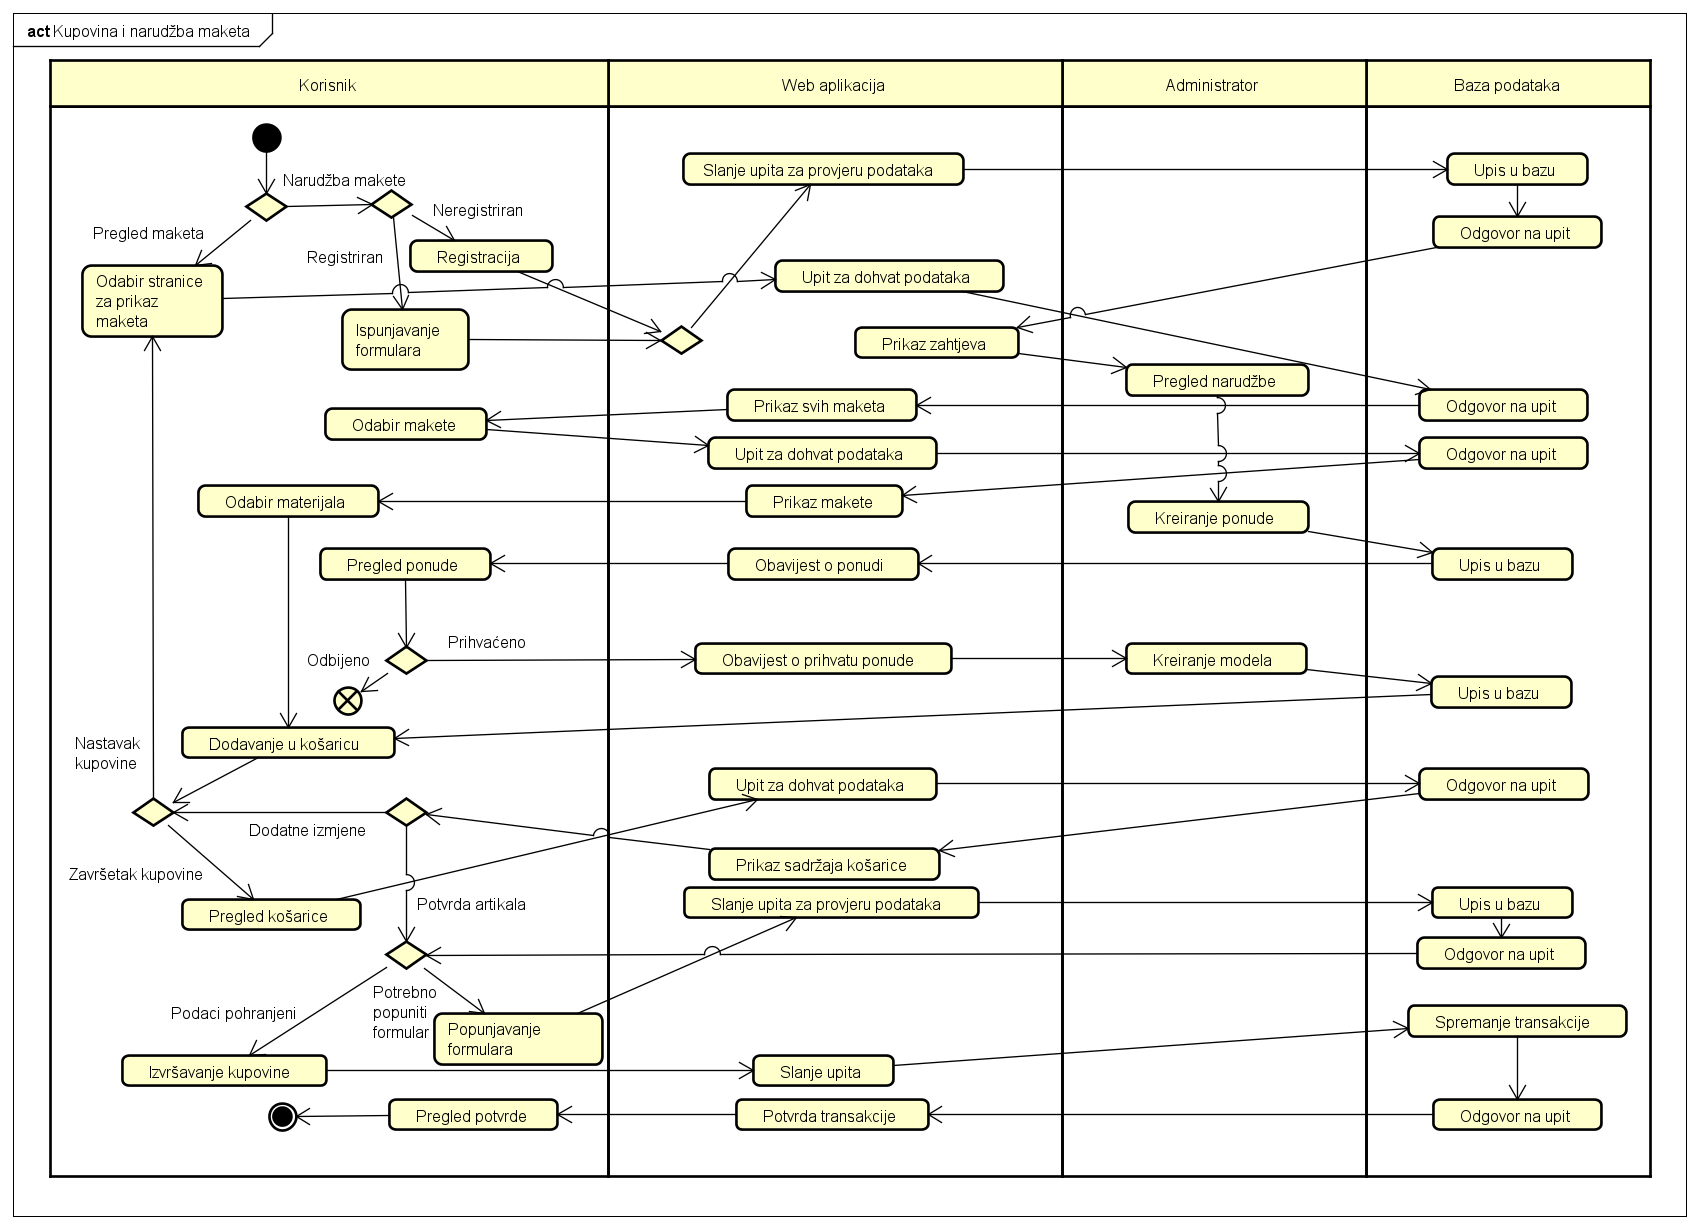
\includegraphics[width=1\linewidth]{slike/Dijagram_aktivnosti_2.PNG} %veličina u odnosu na širinu linije
				\caption{Dijagram aktivnosti za kupovinu i narudžbu maketa}
				\label{fig:diakt2} %label mora biti drugaciji za svaku sliku
			\end{figure}
			
			\eject
		\section{Dijagram komponenti}
			
			Dijagram komponenti služi za prikaz organizacije i interakcije između komponenata implementacije te odnos programske potpore prema okolini. Oblikovanje sustava mora biti dovršeno prije nego se počnu modelirati komponente. Autentifikacija korisnika podrazumijeva mogućnost prijave i registracije novog korisnika. Korisnik
može pregledavati ponuđene makete i nakon toga ih dodavati po potrebi u košaricu. Također postoji mogućnost narudžbe makete prema korisnikovim preferencijama i vlastitim skicama vezano uz veličinu, boju, materijal izrade itd. Opcija naručivanja maketa predviđena je samo za registrirane korisnike.
			
			\begin{figure}[H]
				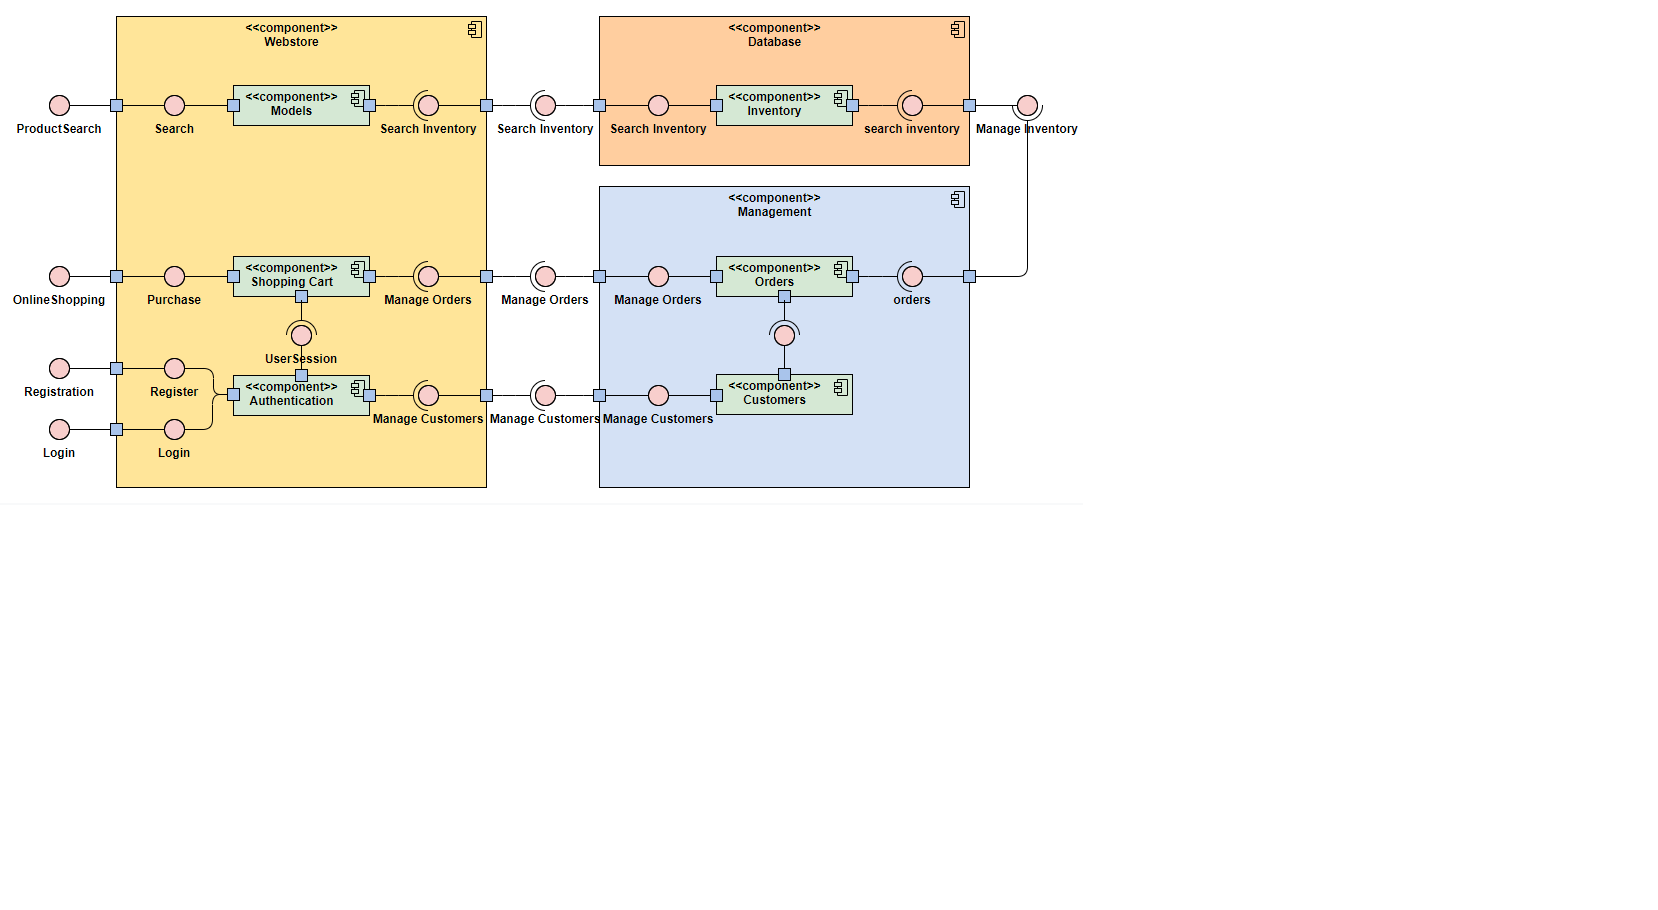
\includegraphics[width=1\linewidth]{slike/dijagram_komponenti.PNG} %veličina u odnosu na širinu linije
				\caption{Dijagram komponenti}
				\label{fig:dijkomp} %label mora biti drugaciji za svaku sliku
			\end{figure}
			
			
			\eject
